% small.tex
\RequirePackage{atbegshi}

\documentclass{beamer}
\usetheme[height=7mm]{Rochester}

\usepackage{graphicx}
\usepackage{hyperref}
\usepackage{skull}
\usepackage{verbatim}
\usepackage[utf8]{inputenc} 
\usepackage[T1]{fontenc}
\usepackage[czech,english]{babel}


\title{OSy: Demín, Marek}
\author{Michal Demín, Kuba Marek}
\date{}

\begin{document}

\frame[plain]{\titlepage}

\begin{frame}{Intro}

Motivation:
\begin{itemize}
\item Robot controller for Eurobot, etc.
\item Need robust platform to handle all tasks
\item Bus for communication among components
\end{itemize}

We chose:
\begin{itemize}
\item Beagleboard
\item Controller Area Network - CAN
\end{itemize}
\end{frame}

\begin{frame}{Beagleboard}
\begin{columns}[c]

\column{.45\textwidth}
:-)
\begin{itemize}
\item OMAP3530 - Cortex-A8, 600MHz
\item 128MB RAM/Flash,
\item 2x SPI bus 
\item 1x I2C bus 
\item SD-card slot
\item USB OTG
\item UART, HDMI, audio, \ldots
\end{itemize}

\column{.55\textwidth}
\includegraphics[width=\textwidth]{../img/beagleboard}

\end{columns}
\end{frame}

\begin{frame}{Beagleboard}
\begin{columns}[c]

\column{.45\textwidth}
:-(
\begin{itemize}
\item No RTC
\item No network connectivity
\item No CAN
\end{itemize}

\column{.55\textwidth}
\includegraphics[width=\textwidth]{../img/beagleboard}

\end{columns}
\end{frame}

\begin{frame}{Expansion Board}
\centering{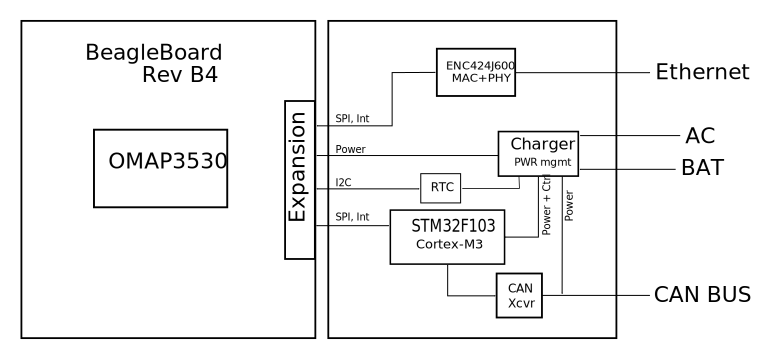
\includegraphics[height=.5\textheight]{../img/system}}
\begin{itemize}
	\item RTC with battery
	\item 10/100Mbit Ethernet (ENC424J600)
	\item STM32 MCU (Cortex-M3 based) \begin{itemize}
	\item CAN bus
	\item Battery/power management
\end{itemize}
\item Exposes more BB peripherals - UART, I2C
\end{itemize}
\end{frame}

\begin{frame}{What did we do}

\begin{columns}[c]
\column{.4\textwidth}

\begin{itemize}
	\item Firmware for embedded MCU
	\item Counterpart driver for embedded MCU 
	\item Ethernet driver
	\item Minor U-Boot modifications
\end{itemize}

\column{.6\textwidth}
\includegraphics[width=\textwidth]{../img/main}

\end{columns}
\end{frame}

\begin{frame}{Embedded MCU - SPI communication}
Protocol rewritten from scratch 2 times

Version 1:
\begin{itemize}
	\item 1 byte command + dummy byte + data
	\item dummy byte = time to process command
	\item Impossible to synchronize MCU with Beagleboard.
\end{itemize}

Version 2 - current:
\begin{itemize}
\item 1 byte command, ACK from MCU, then data
\item Added dedicated interrupt (GPIO) for ACK
\end{itemize}
\end{frame}

\begin{frame}{Embedded MCU - CAN}
\begin{itemize}
	\item Internal bxCAN hardware (3 message RX fifo, 3 TX mailboxes)
	\item Implements 16 message buffer, for message bursts 
	\item Fully interrupt based.
\end{itemize}

\begin{itemize}
\item Bug in HW causes false error reporting :-(
\item Possible speed improvement by preloading messages into TX mailboxes 
\end{itemize}
\end{frame}

\begin{frame}{Embedded MCU - Power}
\begin{itemize}
	\item Uses internal ADC to measure
	\begin{itemize}
		\item Battery voltage
		\item Battery current
		\item System current
		\item AC Power
	\end{itemize}
	\item DMA transfers to offload CPU
	\item PWM to set charging current
	\item Provides interrupts on Battery low, AC present
	\item Glitch-free AC \(\Leftrightarrow\) Battery switch
\end{itemize}
\end{frame}

\begin{frame}{Kernel counterpart driver}
\begin{itemize}
	\item CAN through SocketCAN (netdev)
	\item Power through Linux Power API
	\item Some additional features available only as /sys entry

	\item All communication through SPI
	\item Two interrupts - interrupt and data ack line

	\item CAN is available as network interface (ifconfig can0 up)
\end{itemize}
\end{frame}

\begin{frame}{Microchip ENC424J600}
\begin{itemize}
	\item Fast Ethernet Controller
	\item Integrated MAC and PHY
	\item 24kB SRAM (TX and RX buffers)
	\item HW crypto engines (AES, MD5, SHA1, \ldots)
	\item SPI and parallel interface
	\item Designed specifically for embedded devices
\end{itemize}

\end{frame}

\begin{frame}{Microchip ENC424J600 -- kernel driver}
\begin{itemize}
	\item Straightforward implementation
	\item Supported features
	\begin{itemize}
		\item 10/100Mbit
		\item Full/half duplex
		\item Low-power mode
		\item Autonegotiation
	\end{itemize}
	\item UDP throughput: ~12Mbit
	\item TCP throughput: ~2.5Mbit
	\item SPI is performance bottleneck (14Mbit/s raw)
	\item Slight improvement of TX performance possible (\( < 10\%\))
	\item Developed on stable 2.6.29 kernel
	\item Forked by Indian programmer and rejected from mainline :-)
\end{itemize}
\end{frame}

\begin{frame}{U-boot}
\begin{itemize}
	\item Bootloader for ARM and other processors
	\item Initializes basic HW and sets up pin multiplexing
	\item Pin muxing changed to support our expansion board
	\item Careful when replacing! Leads to bricked HW
\end{itemize}
\end{frame}

\begin{frame}{Board info}
\begin{itemize}
	\item Specify peripherials of the CPU
	\item SPI, interrupt pins, I2C, GPIO
	\item Modified from beagleboard default
\end{itemize}
\end{frame}

\begin{frame}{Lessons learned}
\begin{itemize}
	\item Time time time :-)
	\item Nested interrupts are evil \(\skull\)
	\item Protocol design is crucial
	\item "Read and clear"
	\item GPIO\_148 is not GPIO\_149
\end{itemize}
\end{frame}

\begin{frame}{The end}
\begin{center}
Questions?
\end{center}
\end{frame}

\end{document}
